% ============================================================================
% 附录 AY：聚变材料与辐照损伤 —— 从 dpa 到肿胀与寿命（注明出处）
%
% 数值来源：tools/calc/appAY_calc.py（只打印，输出 tools/calc/appAY_calc.txt）。
%   * 工作点 D1 与附录 M/S/U/V/W/AK/AP/AV/AX 同口径：
%     P_fus = 556.5 MW、P_n = 445.175 MW、A_wall = 489.532 m^2、V = 832.2 m^3。
%   * 中子壁负载取附录 AV/Z 的 0.909388 MW/m^2（由 P_n/A_wall 复算为 0.909389，
%     差 1 个单位来自四舍五入，正文用声明值）。
%   * 材料与损伤侧的声明输入：14 MeV 中子 NRT 位移截面 7.0e-25 m^2（7000 b）、
%     铁基材料离位阈能 40 eV、氦产生率 12 appm/dpa、肿胀孵化期 10 dpa、
%     肿胀速率 0.2 %/dpa、设计剂量上限 50 dpa（上限口径 70 dpa）、
%     硬化饱和增量 400 MPa（饱和尺度 0.1 dpa）、DBTT 位移系数 0.4 K/MPa、
%     未辐照 DBTT -60 摄氏度、溅射产额 1.0e-3、偏滤器氘通量 1e23 m^-2 s^-1、
%     再沉积份额 0.95、钨装甲 5 mm、E = 200 GPa、alpha = 12e-6 /K、nu = 0.3、
%     屈服强度 550 MPa、热循环 3000 次/年、100 MPa/550 摄氏度下蠕变寿命 1e5 h。
%   * 单位口径：dpa（每个原子的离位次数）、appm（百万分之一原子比）、
%     fpy（full power year，3.15576e7 s）、STP（0 摄氏度、101325 Pa）。
%
% 这一篇讲什么：
%   * 附录 Z 给堆的总账（中子壁负载、包层、屏蔽、热工）；
%   * 附录 AK 讲安全与环境（活化、衰变热、氚释放）；
%   * 附录 AP 讲维护与更换周期（这里是它 50.001 dpa 口径的材料侧依据）；
%   * 附录 AV 讲氚循环（本附录只在中子谱与嬗变处交叉引用）；
%   * 本附录补的是「结构材料自己怎么坏」：位移损伤、氦与气泡、肿胀、
%     硬化与脆化、溅射侵蚀、热疲劳与蠕变。
%
% 版权口径：只借经典教材与公开技术文件的公式形式与量级判据，
%   不复制任何成段文字、原图或材料数据库；逐节注明「出处：」。
% ============================================================================

\section{一块钢要同时挨三件事：dpa、氦与热循环}
\label{sec:app-ay-three}

聚变堆的第一壁与包层结构材料，在整个寿命里同时承受三件性质完全不同的事：
\textbf{中子把它撞坏}（位移损伤，单位 dpa）、\textbf{嬗变往它里面塞气}
（氦与氢，单位 appm）、\textbf{热循环让它胀缩}（热应力与疲劳，单位 K 与次数）。
三件事的时间尺度、空间尺度和失效方式都不一样，却必须在同一块钢里同时满足。

先看量级。本书工作点（附录 Z/AV）的中子壁负载是 $0.909388\ \mathrm{MW\,m^{-2}}$，
设计剂量上限取 $50\ \mathrm{dpa}$，运行温度约 $500$ 摄氏度：

\begin{table}[htbp]
\centering
\small
\setlength{\tabcolsep}{4pt}
\begin{tabular}{p{2.4cm}p{3.0cm}p{3.4cm}p{4.6cm}}
\toprule
损伤类型 & 驱动量 & 本附录工作点的量级 & 后果 \\
\midrule
位移损伤 & 中子通量 $\times$ 位移截面 & $8.91268$ dpa/fpy & 硬化、脆化、肿胀 \\
嬗变产气 & $(n,\alpha)$ 反应率 & $12$ appm He/dpa & 气泡、晶界脆化 \\
热循环 & 薄壁温差与次数 & $342.857$ MPa（$\Delta T=100$ K） & 疲劳裂纹 \\
\bottomrule
\end{tabular}
\caption{同一块结构材料上的三种损伤：驱动量、量级与后果。}
\label{tab:app-ay-three}
\end{table}

\textbf{三件事不能分开算}，因为它们互相放大：位移损伤产生空位与间隙原子，
氦偏偏不溶于钢、只往空位团里钻，空位团长大成空洞就是肿胀；
肿胀改变尺寸又改变热应力，而脆化让材料对热应力的容忍度下降。
工程上用一条叠加判据做初筛：

\begin{equation}
\frac{D}{D_\mathrm{lim}}+\frac{c_\mathrm{He}}{c_\mathrm{He,lim}}
+\frac{N}{N_\mathrm{f}}+\frac{t}{t_\mathrm{creep}}\le 1,
\label{eq:app-ay-books}
\end{equation}

其中 $D$ 是累积剂量、$c_\mathrm{He}$ 是氦浓度、$N$ 是热循环次数、$t$ 是运行时间。
四项分别对应本附录的 AY.2--AY.7 六节。

\begin{tip}{三件事不能分开算，但它们的时间尺度差得很远}{tip-app-ay-three}
dpa 是随通量线性累积的（$\sim$ 年），氦也是线性累积的（$\sim$ 年），
肿胀却有一个 $\sim$ 年的孵化期，热循环则是每次脉冲发生一次（$\sim$ 秒）。
做寿命评估时不能说「先算最严重的那一项」——要按时间轴把四条曲线画在一起，
看谁先碰到自己的限值。
\end{tip}

{\footnotesize
\textbf{出处：}三类损伤的划分、dpa 与 appm 的口径、叠加判据的写法参照
Was 的核材料教材与 Zinkle 等的聚变材料综述。
本书只借分类与量级判据，
不复制其损伤演化模型与材料数据库。
}

\begin{figure}[htbp]
\centering
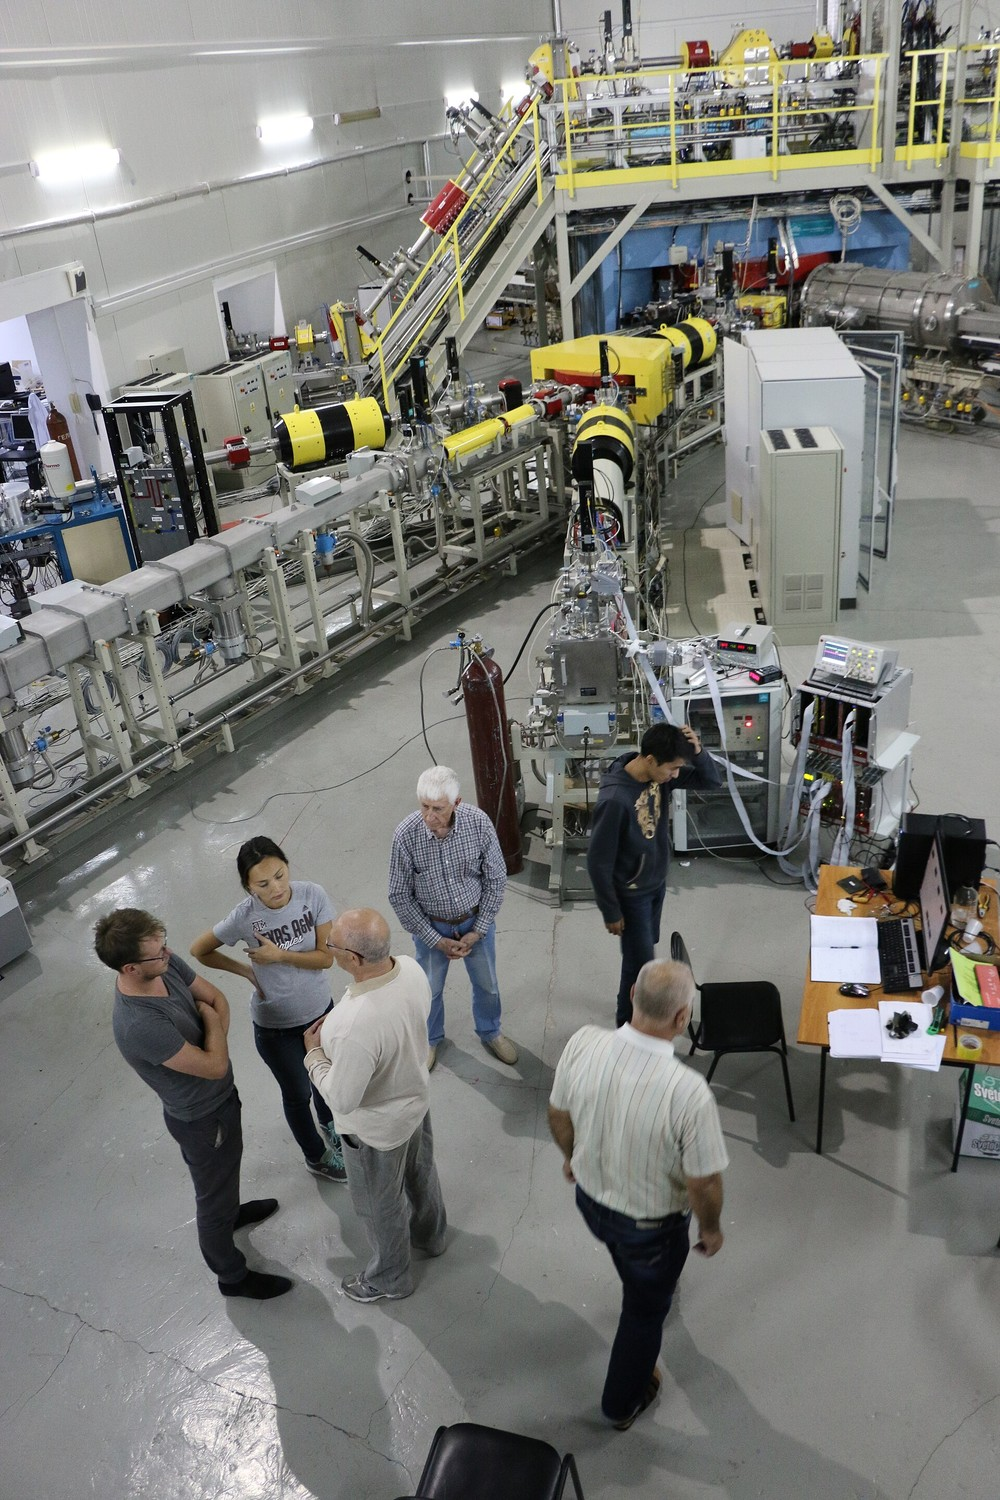
\includegraphics[width=0.60\textwidth]{../figures/ion_irradiation.jpg}
\caption{把位移损伤做出来：离子辐照实验。聚变中子造成的位移损伤要几十年才积累到几个 dpa，实验室里用重离子加速器把它压缩到几天：这就是本章 dpa 计算式的实验对应物。}
\label{fig:photo-appay2}
\figsource{BibMak，CC BY-SA 4.0（Wikimedia Commons），链接见 figures/CREDITS.md。}
\end{figure}

\section{位移损伤：dpa 是怎么从通量算出来的}
\label{sec:app-ay-dpa}

\textbf{dpa}（displacements per atom，每个原子的离位次数）不是能量，也不是剂量率，
而是一个\textbf{计数}：在辐照的时间里，平均每个原子被撞离自己格点几次。
它由中子通量乘一个截面得到，这个截面叫\textbf{位移截面} $\sigma_d$：

\begin{equation}
\Gamma_n=\frac{P_n}{A_\mathrm{wall}E_n}
=\frac{445.175\ \mathrm{MW}}{489.532\ \mathrm{m^2}\times14.068\ \mathrm{MeV}}
=4.03466\times10^{17}\ \mathrm{n\,m^{-2}\,s^{-1}},
\label{eq:app-ay-flux}
\end{equation}

\begin{equation}
\frac{\mathrm{d}D}{\mathrm{d}t}=\sigma_d\Gamma_n
=7.0\times10^{-25}\ \mathrm{m^2}\times4.03466\times10^{17}
=2.82426\times10^{-7}\ \mathrm{dpa\,s^{-1}},
\label{eq:app-ay-dpa}
\end{equation}

\begin{equation}
\begin{aligned}
D_\mathrm{fpy}&=2.82426\times10^{-7}\times3.15576\times10^{7}
=8.91268\ \mathrm{dpa/fpy},\\
\frac{D_\mathrm{fpy}}{0.909388}&=9.80075\ \mathrm{dpa/fpy\ per\ MW\,m^{-2}}.
\end{aligned}
\label{eq:app-ay-fpy}
\end{equation}

最后一行是工程上最常用的拇指规则：\textbf{每 $1\ \mathrm{MW\,m^{-2}}$ 的中子壁负载，
一年全功率运行约对应 $9.8$ dpa}。本附录工作点是 $0.909388\ \mathrm{MW\,m^{-2}}$，
所以到 $50$ dpa 的寿命是

\begin{equation}
t_{50}=\frac{50}{8.91268}=5.60998\ \mathrm{fpy}
=1.77038\times10^{8}\ \mathrm{s},
\qquad
t_{70}=\frac{70}{8.91268}=7.85398\ \mathrm{fpy},
\label{eq:app-ay-life}
\end{equation}

五年全功率运行累积 $44.5634$ dpa，是上限的 $89.1268\%$——也就是说，
\textbf{结构材料的寿命不是「几十年」，而是「五到八年」}，这直接决定了
附录 AP 的包层更换周期。

位移截面 $7.0\times10^{-25}\ \mathrm{m^2}=7000$ b 是怎么来的？
NRT 模型把它拆成两步：中子先撞出一个初级离位原子（PKA），
PKA 再在级联里撞出 $N_\mathrm{NRT}$ 个离位，于是

\begin{equation}
N_\mathrm{NRT}=\frac{0.8\,E_\mathrm{damage}}{2E_d},
\qquad
\sigma_d=N_\mathrm{NRT}\,\sigma_\mathrm{PKA},
\label{eq:app-ay-nrt}
\end{equation}

其中 $E_d=40$ eV 是铁基材料的离位阈能，$0.8$ 是 NRT 的效率因子。
$E_\mathrm{damage}$ 是 14 MeV 中子产生的平均损伤能（几十 keV 量级），
$N_\mathrm{NRT}$ 因此是几百到上千——\textbf{一个中子能撞飞一千个原子}，
这就是聚变中子「毒性」的第一层含义。

每 $1$ dpa 对应的通量是一个常用换算：

\begin{equation}
\Phi_{1\,\mathrm{dpa}}=\frac{1}{\sigma_d}
=\frac{1}{7.0\times10^{-25}}=1.42857\times10^{24}\ \mathrm{n\,m^{-2}}.
\label{eq:app-ay-fluence}
\end{equation}

\begin{table}[htbp]
\centering
\small
\setlength{\tabcolsep}{4pt}
\begin{tabular}{p{4.4cm}p{3.0cm}p{3.6cm}p{2.4cm}}
\toprule
量 & 符号 & 本工作点数值 & 单位 \\
\midrule
中子壁负载 & $P_n/A_\mathrm{wall}$ & $0.909388$ & MW\,m$^{-2}$ \\
中子通量 & $\Gamma_n$ & $4.03466\times10^{17}$ & n\,m$^{-2}$\,s$^{-1}$ \\
dpa 率 & $\mathrm{d}D/\mathrm{d}t$ & $2.82426\times10^{-7}$ & dpa\,s$^{-1}$ \\
年累积 & $D_\mathrm{fpy}$ & $8.91268$ & dpa/fpy \\
单位壁负载 & --- & $9.80075$ & dpa/fpy per MW\,m$^{-2}$ \\
到 50 dpa & $t_{50}$ & $5.60998$ & fpy \\
到 70 dpa & $t_{70}$ & $7.85398$ & fpy \\
5 年累积 & $5D_\mathrm{fpy}$ & $44.5634$（$89.1268\%$） & dpa \\
每 1 dpa 对应通量 & $1/\sigma_d$ & $1.42857\times10^{24}$ & n\,m$^{-2}$ \\
\bottomrule
\end{tabular}
\caption{位移损伤的完整换算链：从中子壁负载到寿命。}
\label{tab:app-ay-dpa}
\end{table}

\begin{tip}{dpa 是计数，不是能量}{tip-app-ay-dpa}
经常有人把 dpa 当成「吸收了多少能量」。不是：dpa 说的是
\textbf{每个原子平均被撞离位几次}。同样 1 dpa，14 MeV 中子、
裂变中子和重离子造成的级联形态完全不同（级联越大，空位团越集中，
越容易长成空洞），所以材料界才有「同样的 dpa、不同的损伤」这句话。
工程上还常用「dpa 只算 NRT、不算氦」的做法，本附录后面要说明
为什么这在聚变里不够。
\end{tip}

{\footnotesize
\textbf{出处：}dpa 的定义、NRT 模型与位移截面的量级口径参照
Was 的核材料教材、Norgert--Robinson--Torrens 的 NRT 原文与
Gilbert 等的聚变中子损伤截面工作。
本书只借定义与量级判据，
不复制其级联模拟程序与截面数据表。
}

\section{氦与氢：聚变中子为什么比裂变中子更毒}
\label{sec:app-ay-he}

同样产生 $1$ dpa，聚变中子制造的氦比裂变中子多一到两个数量级：
14 MeV 中子能量高于铁、铬、钨的 $(n,\alpha)$ 与 $(n,p)$ 反应阈能，
每一级联里都顺手产气。声明氦产生率 $12$ appm/dpa，
则 $50$ dpa 后氦浓度是

\begin{equation}
c_\mathrm{He}=12\ \mathrm{appm/dpa}\times50\ \mathrm{dpa}
=600\ \mathrm{appm}=0.06\ \mathrm{at.\%},
\label{eq:app-ay-he}
\end{equation}

把两个产生率写成比值，就得到聚变中子谱的一个特征数：

\begin{equation}
\frac{c_\mathrm{He}}{D}=12\ \mathrm{appm/dpa}
\quad\Longleftrightarrow\quad
\frac{1\ \mathrm{dpa}}{1.42857\times10^{24}\ \mathrm{n\,m^{-2}}}
\ \text{对应}\ 12\ \mathrm{appm}\ \mathrm{He}.
\label{eq:app-ay-ratio}
\end{equation}

$0.06$ at.\% 听上去微不足道，但\textbf{氦在钢里几乎不溶}：
它的固溶度极低，几乎所有氦原子都会汇聚成气泡。把钢的原子密度
取 $8.46518\times10^{28}\ \mathrm{m^{-3}}$（$\rho=7850\ \mathrm{kg\,m^{-3}}$、
$M=0.055845\ \mathrm{kg\,mol^{-1}}$），$600$ appm 对应
$5.07911\times10^{25}\ \mathrm{m^{-3}}$ 个氦原子；
把这些氦全部按标准状态折算成气体，体积是

\begin{equation}
V_\mathrm{STP}=\frac{n_\mathrm{He}}{N_A}\times22.41397\times10^{-3}
=1.89041\ \mathrm{m^3}=1890.41\ \mathrm{L}
\quad(\text{每立方米钢}),
\label{eq:app-ay-stp}
\end{equation}

也就是说，\textbf{一块一立方米的钢里塞进了将近两千升的氦气}。
这些氦不会老老实实待着：小的氦-空位团在几百摄氏度就能迁移、合并，
最终形成纳米级气泡。半径为 $1$ nm 的气泡，靠表面张力就能维持

\begin{equation}
p=\frac{2\gamma}{r}=\frac{2\times1.0\ \mathrm{J\,m^{-2}}}{1.0\times10^{-9}\ \mathrm{m}}
=2.0\times10^{9}\ \mathrm{Pa}=2\ \mathrm{GPa}
\label{eq:app-ay-bubble}
\end{equation}

的内压——是运行应力（几十 MPa）的几十倍。$2$ GPa 的局部内压足以把周围的
晶格推开、并在晶界上把气泡连成裂纹，这就是\textbf{氦脆}。

\begin{table}[htbp]
\centering
\small
\setlength{\tabcolsep}{4pt}
\begin{tabular}{p{4.6cm}p{3.2cm}p{3.4cm}p{2.2cm}}
\toprule
量 & 符号 & 数值 & 单位 \\
\midrule
钢的原子密度 & $n_\mathrm{steel}$ & $8.46518\times10^{28}$ & m$^{-3}$ \\
氦产生率 & $c_\mathrm{He}/D$ & $12$ & appm/dpa \\
50 dpa 后氦浓度 & $c_\mathrm{He}$ & $600$（$0.06$ at.\%） & appm \\
44.5634 dpa 时 & $c_\mathrm{He}$ & $534.762$ & appm \\
氦原子密度 & $n_\mathrm{He}$ & $5.07911\times10^{25}$ & m$^{-3}$ \\
折算气体体积 & $V_\mathrm{STP}$ & $1.89041$（$1890.41$ L） & m$^3$/m$^3$ \\
1 nm 气泡内压 & $2\gamma/r$ & $2.0\times10^{9}$（$2$ GPa） & Pa \\
\bottomrule
\end{tabular}
\caption{氦的账：从 appm 到「每立方米近两千升气体」再到气泡内压。}
\label{tab:app-ay-he}
\end{table}

\begin{tip}{氦不溶，所以它只往气泡里跑}{tip-app-ay-helium}
氦原子在金属里的固溶度低到可以忽略，这意味着它\textbf{没有「留在晶格里」这个选项}：
要么被空位抓住形成团簇，要么被晶界、位错捕集。于是氦的破坏方式
与「固溶强化」完全不同——它不是把晶格撑硬，而是
\textbf{在晶界上把材料拆开}。聚变材料设计里很多巧妙办法
（纳米析出相、晶界工程、氧化物弥散强化）本质上都是在给氦
提供「无害的落脚点」。
\end{tip}

{\footnotesize
\textbf{出处：}聚变中子的 $(n,\alpha)$/$(n,p)$ 反应、氦产生率的 appm/dpa 量级
与氦脆机理参照 Zinkle、Odette 等的聚变材料综述与 Was 的教材。
标准状态气体体积换算用本书附录 D 的单位常数。
本书只借机理与量级，
不复制其气泡演化动力学模型与实验数据。
\section{肿胀：剂量、温度与孵化期}
\label{sec:app-ay-swell}
}

位移损伤产生空位与间隙原子。间隙原子跑得快、很快被位错吸收；
空位跑得慢，容易聚成空位团。如果空位团里再被氦稳住，它就不会解散，
而是越长越大成为\textbf{空洞}（void）——材料因此\textbf{体积膨胀}，这就是肿胀。

肿胀不是从第一 dpa 就开始的：它有一个\textbf{孵化期}（incubation），
在孵化期内空位团的尺寸还没到能稳定长大的临界值。用最简的线性段模型，
声明孵化期 $D_\mathrm{inc}=10\ \mathrm{dpa}$、肿胀速率 $0.2\ \%/\mathrm{dpa}$：

\begin{equation}
\frac{\Delta V}{V}=
\begin{cases}
0, & D<D_\mathrm{inc},\\[2pt]
s\,(D-D_\mathrm{inc}), & D\ge D_\mathrm{inc},
\end{cases}
\qquad
s=0.2\ \%/\mathrm{dpa},\quad D_\mathrm{inc}=10\ \mathrm{dpa},
\label{eq:app-ay-swell}
\end{equation}

在 $50$ dpa 时

\begin{equation}
\frac{\Delta V}{V}=0.2\times(50-10)=8.0\ \%,
\qquad
\frac{\Delta L}{L}=(1.08)^{1/3}-1=2.59856\ \%,
\label{eq:app-ay-line}
\end{equation}

上式的第二个等号是很多人忽略的一步：\textbf{体积肿胀 $8\%$ 对应线性尺寸变化
$2.6\%$}，而不是 $8\%$。包层模块之间必须留出这段间隙，否则相邻模块会互相顶住。
到 $70$ dpa 时肿胀是 $12\%$，线性变化 $3.85\%$。五年的实际运行（$44.5634$ dpa）
对应 $6.91268\%$。

孵化期还有一个容易漏掉的含义：\textbf{它把剂量变成了时间}。
$10$ dpa 的孵化期折合 $1.122$ fpy——也就是说，一块材料在前一年多的时间里
看不出任何肿胀，然后才开始以 $0.2\%$/dpa 的速度长胖。
用「$1\%$ 肿胀」作为报警线，所需剂量是 $15$ dpa（约 $1.68299$ fpy）。

\begin{table}[htbp]
\centering
\small
\setlength{\tabcolsep}{4pt}
\begin{tabular}{p{4.4cm}p{2.6cm}p{2.8cm}p{3.4cm}}
\toprule
量 & 剂量 & 肿胀（体积） & 线性尺寸变化 \\
\midrule
孵化期结束 & $10$ dpa & $0$ & $0$ \\
五年运行 & $44.5634$ dpa & $6.91268\%$ & $2.25308\%$ \\
设计上限 & $50$ dpa & $8.0\%$ & $2.59856\%$ \\
上限口径 & $70$ dpa & $12.0\%$ & $3.84988\%$ \\
$1\%$ 报警线 & $15$ dpa & $1.0\%$ & $0.332228\%$ \\
\bottomrule
\end{tabular}
\caption{肿胀的线性段模型：孵化期、五年运行、设计上限与报警线。}
\label{tab:app-ay-swell}
\end{table}

\begin{tip}{肿胀有孵化期，所以「前两年没事」不是好消息}{tip-app-ay-swelling}
材料的失效往往发生在「看起来一直很好」之后。肿胀的孵化期、氦泡的孕育期、
辐照脆化的饱和期都有类似形状：\textbf{先是一段几乎没有变化的平台，
然后拐弯}。工程上不能用平台段去外推寿命——那正是设计评审里
最容易被追问的一条。反过来，如果把运行温度、成分与初始组织设计好
（例如氧化物弥散强化钢、纳米析出相），孵化期可以被显著拉长，
这就是「抗肿胀材料」的核心思路。
\end{tip}

{\footnotesize
\textbf{出处：}空洞肿胀的孵化期—线性段描述、温度依赖与抗肿胀组织设计
参照 Was 的核材料教材、Zinkle 与 Odette 的聚变材料综述。
本书只借唯象模型与量级，不复制其速率理论推导与辐照实验数据。
}

\section{辐照硬化与脆化：DBTT 位移意味着什么}
\label{sec:app-ay-hard}

位移损伤产生的缺陷团与位错环会\textbf{钉住位错}，材料的屈服强度因此升高——
这叫辐照硬化。硬化的坏处不是「更硬」，而是\textbf{更脆}：
屈服强度升高、均匀延伸率下降，韧脆转变温度（DBTT）向高温移动。
用饱和型模型描述，声明饱和增量 $\Delta\sigma_\mathrm{sat}=400$ MPa、
饱和尺度 $d_0=0.1$ dpa：

\begin{equation}
\begin{aligned}
\Delta\sigma_y(D)&=\Delta\sigma_\mathrm{sat}
\left[1-\exp\!\left(-\frac{D}{d_0}\right)\right],\\
\Delta\sigma_y(1\ \mathrm{dpa})&=399.982\ \mathrm{MPa},
\qquad
\Delta\sigma_y(0.1\ \mathrm{dpa})=252.848\ \mathrm{MPa}.
\end{aligned}
\label{eq:app-ay-hard}
\end{equation}

注意这两个数：$0.1$ dpa 就已经达到饱和值的 $63.2121\%$，
$1$ dpa 之后基本饱和。\textbf{硬化是「早期事件」}——它在第一年就完成，
而肿胀要等到第二年之后。屈服强度从 $550$ MPa 升到

\begin{equation}
\sigma_y^\mathrm{irr}=\sigma_y+\Delta\sigma_y=550+400=950\ \mathrm{MPa},
\qquad
\frac{\Delta\sigma_y}{\sigma_y}=72.7273\ \%,
\label{eq:app-ay-sum}
\end{equation}

提高 $72.7273\%$，而延伸率往往降到原来的一半以下。

DBTT 的位移用经验系数 $\kappa=0.4\ \mathrm{K/MPa}$ 估算：

\begin{equation}
\Delta T_\mathrm{DBTT}=\kappa\,\Delta\sigma_y
=0.4\times400=160\ \mathrm{K},
\qquad
T_\mathrm{DBTT}^\mathrm{irr}=-60+160=100\ ^\circ\mathrm{C},
\label{eq:app-ay-dbtt}
\end{equation}

也就是说，材料的韧脆转变温度从 $-60$ 摄氏度升到了 $100$ 摄氏度。
工程上要求\textbf{运行温度至少比辐照后的 DBTT 高 $100$ K}，
于是温度下限是 $200$ 摄氏度——这正好是 AY.7 里温度窗口的左端。

\begin{table}[htbp]
\centering
\small
\setlength{\tabcolsep}{4pt}
\begin{tabular}{p{4.6cm}p{2.8cm}p{3.0cm}p{2.6cm}}
\toprule
量 & 符号 & 数值 & 单位 \\
\midrule
饱和硬化增量 & $\Delta\sigma_\mathrm{sat}$ & $400$ & MPa \\
0.1 dpa 时 & $\Delta\sigma_y$ & $252.848$ & MPa \\
1 dpa 时 & $\Delta\sigma_y$ & $399.982$ & MPa \\
50 dpa 时 & $\Delta\sigma_y$ & $400$ & MPa \\
辐照后屈服强度 & $\sigma_y^\mathrm{irr}$ & $950$ & MPa \\
屈服提高比例 & $\Delta\sigma_y/\sigma_y$ & $72.7273$ & \% \\
DBTT 位移 & $\Delta T_\mathrm{DBTT}$ & $160$ & K \\
辐照后 DBTT & $T_\mathrm{DBTT}^\mathrm{irr}$ & $100$ & $^\circ$C \\
运行温度下限 & DBTT $+100$ K & $200$ & $^\circ$C \\
\bottomrule
\end{tabular}
\caption{辐照硬化与脆化：从缺陷钉扎到温度下限。}
\label{tab:app-ay-hard}
\end{table}

\begin{tip}{硬化不是好事：强度与韧性在辐照里是此消彼长的}{tip-app-ay-dbtt}
外行看到「屈服强度从 $550$ MPa 升到 $950$ MPa」会觉得材料变强了。
对结构件来说恰恰相反：\textbf{均匀延伸率与断裂韧性同时下降}，
裂纹更容易在应力集中处萌生并直接扩展。这就是为什么聚变材料
的判据里既有「强度够不够」，也有「DBTT 抬到哪儿」——
而且后者往往先成为限制。
\end{tip}

{\footnotesize
\textbf{出处：}辐照硬化的饱和型描述、缺陷钉扎机理与 DBTT 位移的经验关系
参照 Was 的教材、Odette 与 Lucas 的小尺度硬化模型以及
Zinkle 等的聚变材料综述。
本书只借唯象关系与量级，不复制其
速率理论、断裂韧性数据库与 Master Curve 方法。
}

\begin{figure}[htbp]
\centering
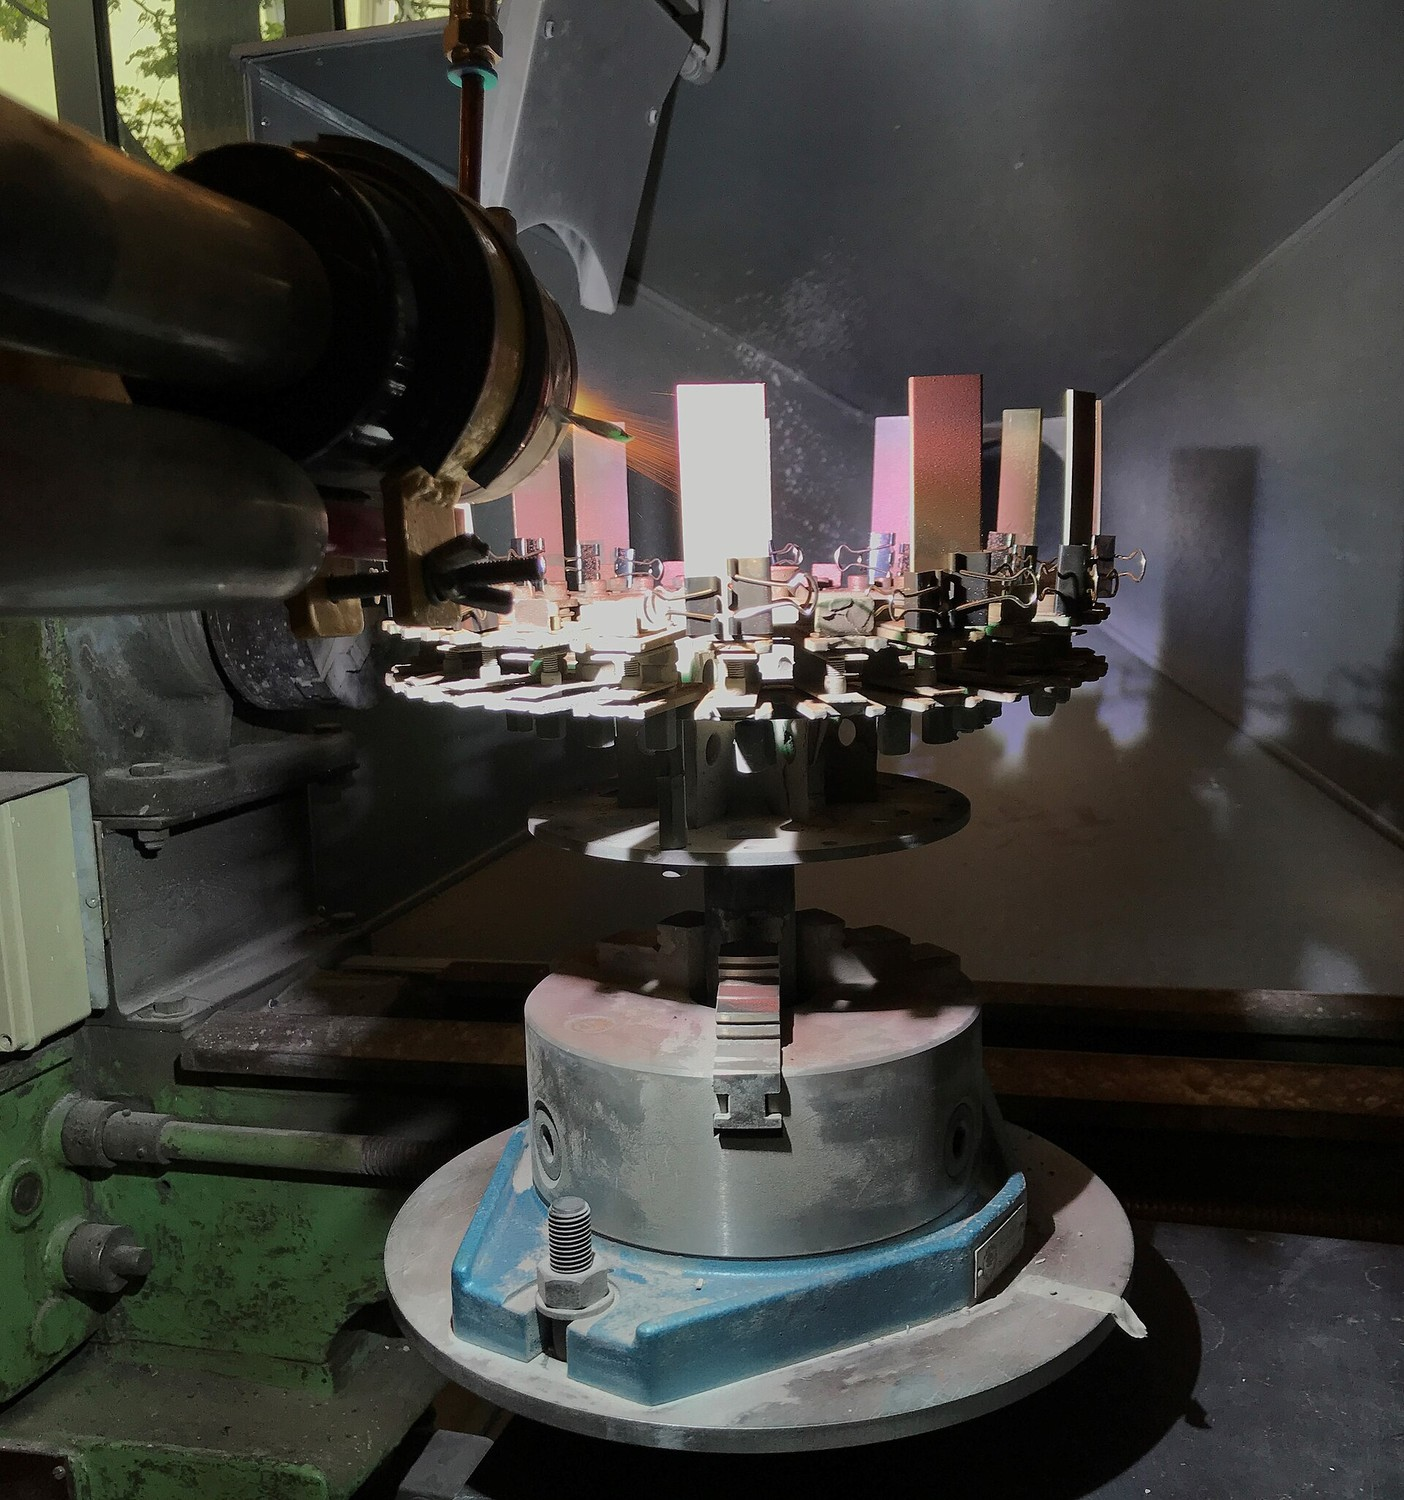
\includegraphics[width=0.72\textwidth]{../figures/plasma_spray.jpg}
\caption{给面向等离子体部件做涂层：等离子体喷涂。喷涂枪里的小型等离子体把粉末熔化并高速打到基体上，形成抗溅射的涂层——这是把本章的「净侵蚀才是寿命」用在工程上的样子。}
\label{fig:photo-appay}
\figsource{Student-julia-pwr，CC BY-SA 4.0（Wikimedia Commons），链接见 figures/CREDITS.md。}
\end{figure}

\begin{figure}[htbp]
\centering
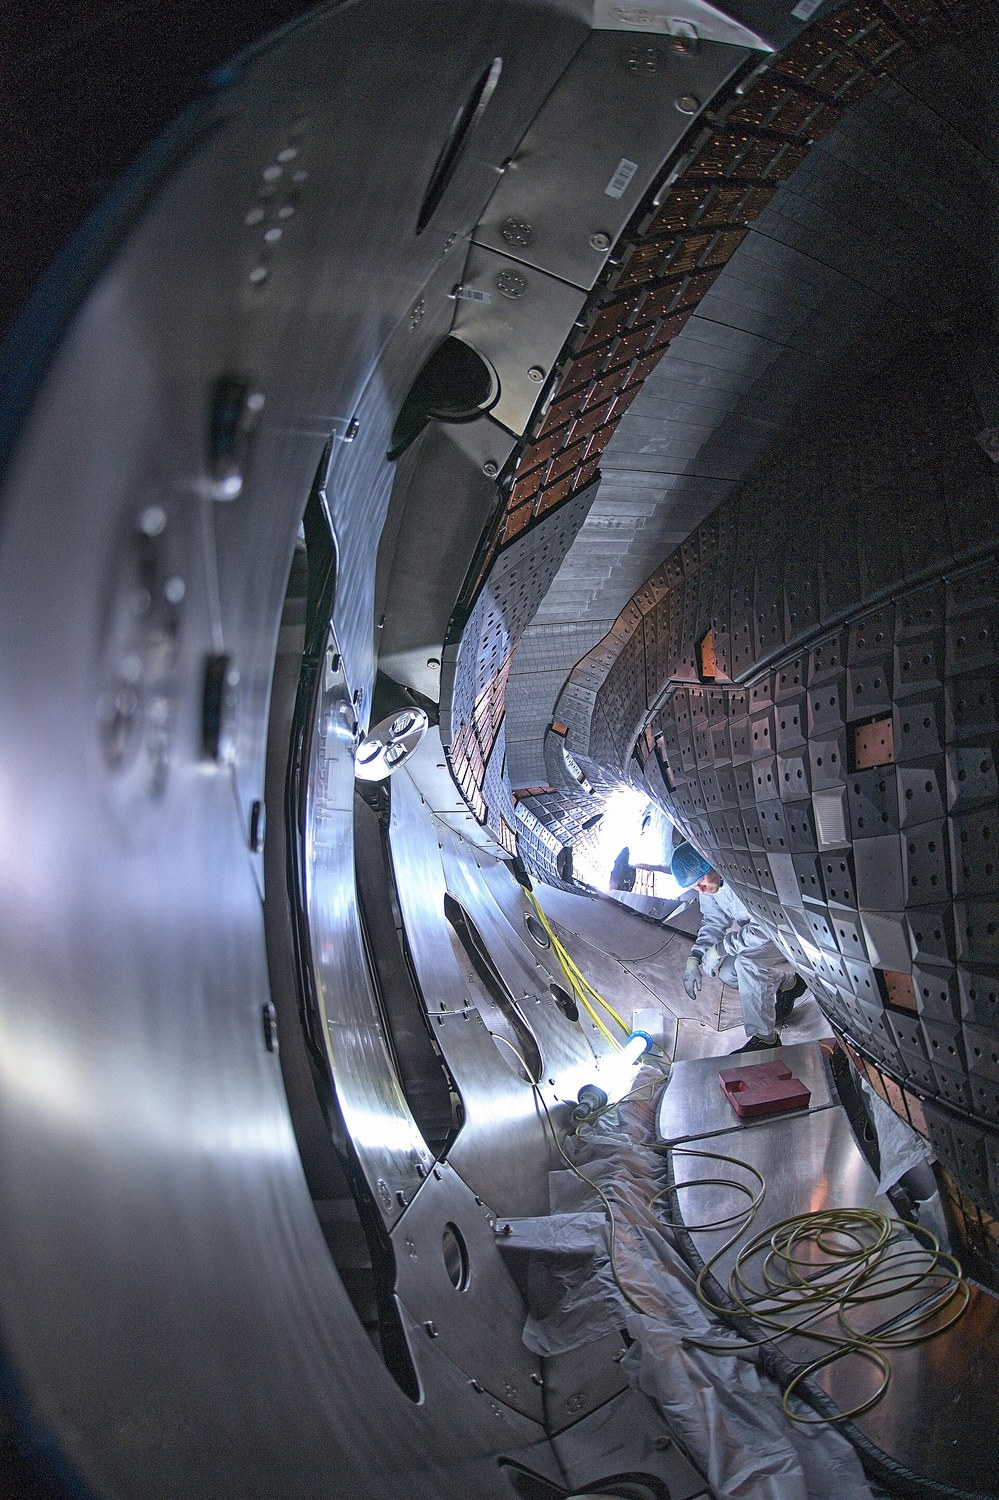
\includegraphics[width=0.60\textwidth]{../figures/ay_w7x_tiles.jpg}
\caption{寿命是数出来的：一块瓦能挨多少热流、被溅射掉多少，决定了整个部件的更换周期。本节算的净侵蚀与热负荷，就落在图中这批主动冷却的偏滤器瓦上。}
\label{fig:photo-appay3}
\figsource{Christopher Roux / EUROfusion，CC BY 4.0（Wikimedia Commons）}
\end{figure}

\section{溅射侵蚀与再沉积：净侵蚀才是寿命}
\label{sec:app-ay-erosion}

结构材料不只被中子从内部打坏，还被等离子体从\textbf{表面}一点点削掉。
偏滤器靶板面对的氘离子通量高达 $10^{23}\ \mathrm{m^{-2}\,s^{-1}}$，
每个离子有一定概率把靶面原子撞出来，这个概率就是\textbf{溅射产额} $Y$。
声明 $Y=1.0\times10^{-3}$（钨，量级口径），总侵蚀速率是

\begin{equation}
R_\mathrm{gross}=\frac{Y\,\Gamma_D M_W}{\rho_W N_A}
=\frac{10^{-3}\times10^{23}\times0.18384}
{19300\times6.02214\times10^{23}}
=1.58173\times10^{-9}\ \mathrm{m\,s^{-1}}=49.9155\ \mathrm{mm/fpy},
\label{eq:app-ay-sput}
\end{equation}

将近 $50$ 毫米每年——如果这是真的，$5$ 毫米的钨装甲只够用一个月。
但溅射出来的钨原子大部分会被等离子体\textbf{电离并送回}靶面，
重新沉积下来。真正的寿命由\textbf{净侵蚀}决定：

\begin{equation}
R_\mathrm{net}=(1-f_\mathrm{redep})R_\mathrm{gross}
=0.05\times49.9155=2.49578\ \mathrm{mm/fpy},
\qquad
t_W=\frac{5.0}{2.49578}=2.00338\ \mathrm{fpy}.
\label{eq:app-ay-net}
\end{equation}

再沉积份额每提高一点，寿命就大幅延长：$f_\mathrm{redep}=0.99$ 时
$t_W=10.0169$ fpy——	extbf{净侵蚀对再沉积份额极其敏感}，
这正是偏滤器几何设计（闭环的靶板结构、私通量区）比材料选择更关键的原因。

\begin{table}[htbp]
\centering
\small
\setlength{\tabcolsep}{4pt}
\begin{tabular}{p{4.6cm}p{2.8cm}p{3.0cm}p{2.6cm}}
\toprule
量 & 符号 & 数值 & 单位 \\
\midrule
溅射产额 & $Y$ & $1.0\times10^{-3}$ & 原子/离子 \\
氘离子通量 & $\Gamma_D$ & $1.0\times10^{23}$ & m$^{-2}$\,s$^{-1}$ \\
总侵蚀速率 & $R_\mathrm{gross}$ & $49.9155$ & mm/fpy \\
再沉积速率 & $f_\mathrm{redep}R_\mathrm{gross}$ & $47.4198$ & mm/fpy \\
净侵蚀速率 & $R_\mathrm{net}$ & $2.49578$ & mm/fpy \\
$5$ mm 装甲寿命 & $t_W$ & $2.00338$ & fpy \\
每 $10^{26}$ 离子 & --- & $0.00158173$ & mm \\
再沉积 $0.99$ 时寿命 & $t_W$ & $10.0169$ & fpy \\
\bottomrule
\end{tabular}
\caption{溅射侵蚀的账：总侵蚀、再沉积与净侵蚀。}
\label{tab:app-ay-erosion}
\end{table}

\begin{tip}{净侵蚀才是寿命，总侵蚀只是「吞吐量」}{tip-app-ay-erosion}
看到 $50$ mm/fpy 的总侵蚀不必惊慌：那些原子绝大多数会回到靶面附近。
工程上真正要控制的是\textbf{净侵蚀}——它由再沉积份额、
打击点扫掠（让热点轮流工作）与几何遮挡共同决定。
反过来说，任何降低净侵蚀的手段（提高再沉积、加宽打击点、
优化磁场构型）都比「换更硬的材料」见效更快，
因为材料侧的溅射产额只有几倍的调节空间，
而再沉积份额可以从 $0.95$ 调到 $0.99$，直接换来 $5$ 倍寿命。
\end{tip}

{\footnotesize
\textbf{出处：}溅射产额的量级、再沉积与净侵蚀的口径参照
ITER 偏滤器公开技术文件、Eckstein 的溅射产额汇编与
Stangeby 的边界等离子体教材。
本书只借量级与判据，
不复制其溅射产额数据表、侵蚀—再沉积模拟程序与靶板几何。
\section{热疲劳与蠕变：温度窗口的两端}
\label{sec:app-ay-window}
}

结构材料的温度不是随便选的：\textbf{太低会脆}（AY.5 的 DBTT 抬到 $100$ 摄氏度，
运行温度至少要比它高 $100$ K），\textbf{太高会蠕变}（RAFM 钢的上限约
$550$ 摄氏度）。中间这段就是\textbf{温度窗口}，本附录工作点取 $500$ 摄氏度。

窗口的右端由蠕变决定：$100$ MPa、$550$ 摄氏度下这种钢的蠕变寿命约
$1.0\times10^{5}$ h，而五年的运行时间是

\begin{equation}
t_\mathrm{mission}=5\times3.15576\times10^{7}\ \mathrm{s}
=43830\ \mathrm{h},
\qquad
\frac{t_\mathrm{creep}}{t_\mathrm{mission}}=\frac{1.0\times10^{5}}{43830}=2.28154,
\label{eq:app-ay-creep}
\end{equation}

余量只有 $2.28154$ 倍——\textbf{蠕变是与 dpa 同量级的寿命限制}，
这在裂变堆里往往不是问题（寿命由中子经济性决定），在聚变堆里却很紧。

窗口的内部还有热应力。第一壁两侧温差 $\Delta T$ 引起的热应力（薄壁约束）是

\begin{equation}
\sigma_\mathrm{th}=\frac{E\alpha\,\Delta T}{1-\nu}
=\frac{200\ \mathrm{GPa}\times12\times10^{-6}\times100\ \mathrm{K}}{0.7}
=342.857\ \mathrm{MPa},
\qquad
\frac{\sigma_\mathrm{th}}{\sigma_y}=0.623377,
\label{eq:app-ay-thermal}
\end{equation}

即 $100$ K 的温差就用掉屈服强度的 $62.3377\%$。这个循环会不会累积塑性应变？
判据是\textbf{弹性安定}：只要热应变不超过两倍屈服应变，结构在几次循环后
就转为纯弹性，不会再累积损伤：

\begin{equation}
\varepsilon_\mathrm{th}=\alpha\Delta T=1.2\times10^{-3},
\qquad
\varepsilon_\mathrm{shakedown}=\frac{2\sigma_y}{E}=\frac{2\times550\ \mathrm{MPa}}{200\ \mathrm{GPa}}
=5.5\times10^{-3},
\qquad
\varepsilon_\mathrm{th}<\varepsilon_\mathrm{shakedown}.
\label{eq:app-ay-shakedown}
\end{equation}

对 $100$ K 的工况，答案是「弹性安定」，所以寿命不由热疲劳决定。
但如果温差大到 $500$ K（例如打击点扫掠失败、局部热流翻几倍），
热应变 $6\times10^{-3}$ 超过安定界限，塑性应变 $5\times10^{-4}$ 开始累积，
用 Coffin--Manson 关系（$\varepsilon_f=0.2$、$c=-0.5$）估算的寿命是

\begin{equation}
N_f=0.5\left(\frac{\varepsilon_\mathrm{pl}}{2\varepsilon_f}\right)^{1/c}
=0.5\left(\frac{5\times10^{-4}}{0.4}\right)^{-2}
=3.2\times10^{5}\ \text{次},
\qquad
N_\mathrm{5y}=3000\times5=15000,
\label{eq:app-ay-cycle}
\end{equation}

余量 $21.3333$ 倍。把三条限制画在一起，就得到完整的\textbf{寿命预算}：

\begin{equation}
\underbrace{\frac{D}{50}}_{\to\ 5.60998\ \mathrm{fpy}}
+\underbrace{\frac{c_\mathrm{He}}{600\ \mathrm{appm}}}_{\text{与 dpa 同步}}
+\underbrace{\frac{N}{N_f}}_{\text{弹性安定，可忽略}}
+\underbrace{\frac{t}{t_\mathrm{creep}}}_{\to\ 2.28154\ \text{倍余量}}
\le\ 1,
\qquad
T\in[200,550]\ ^\circ\mathrm{C}.
\label{eq:app-ay-budget}
\end{equation}

\noindent\textbf{结论：聚变结构材料的寿命由 dpa 与蠕变共同决定，
各给约五到八年；热疲劳只在温差失控时才会成为限制。}

\begin{table}[htbp]
\centering
\small
\setlength{\tabcolsep}{4pt}
\begin{tabular}{p{4.4cm}p{3.0cm}p{3.2cm}p{2.6cm}}
\toprule
限制 & 判据 & 本工作点数值 & 折合寿命 \\
\midrule
位移损伤 & $50$ dpa 上限 & $8.91268$ dpa/fpy & $5.60998$ fpy \\
氦脆 & $600$ appm & 与 dpa 同步 & 同左 \\
蠕变 & $1.0\times10^{5}$ h & $43830$ h（$5$ 年） & 余量 $2.28154$ \\
热疲劳（$100$ K） & 弹性安定 & $\varepsilon_\mathrm{th}=1.2\times10^{-3}$ & 不限制 \\
热疲劳（$500$ K） & $N_f=3.2\times10^{5}$ & $N_\mathrm{5y}=15000$ & 余量 $21.3333$ \\
温度窗口 & DBTT $+100$ K 到 $550$ 摄氏度 & $200$--$550$ 摄氏度 & 宽 $350$ K \\
\bottomrule
\end{tabular}
\caption{四条寿命限制的汇总：谁先到、余量多少。}
\label{tab:app-ay-life}
\end{table}

\begin{tip}{温度窗口是设计出来的，不是自然存在的}{tip-app-ay-window}
很多材料在室温下性能优异，在聚变堆里却完全不能用：\textbf{温度窗口是
「不被辐照脆化」与「不被蠕变拉长」两个约束夹出来的一段区间}，
而这两个约束本身都随辐照变化（DBTT 随剂量升高，蠕变强度随组织演化下降）。
所以材料研发的目标不是「更强的钢」，而是\textbf{更宽、更稳定的温度窗口}——
这也是 RAFM 钢、氧化物弥散强化钢与钨合金三条路线的共同判据。
\end{tip}

{\footnotesize
\textbf{出处：}温度窗口、弹性安定判据、Coffin--Manson 关系与蠕变寿命口径
参照 Was 的教材、Zinkle 与 Odette 的聚变材料综述以及
ITER 结构设计准则的公开技术文件。
本书只借判据形式与量级，
不复制其设计曲线、材料数据库与评定程序。
}

\section{估算练习}
\label{sec:app-ay-problems}

\textbf{练习 1} 若中子壁负载提高到 $2.0\ \mathrm{MW\,m^{-2}}$，
dpa 率是多少？到 $50$ dpa 还能用几年？

\textbf{解答 1} 直接用拇指规则 $9.80075$ dpa/fpy per $\mathrm{MW\,m^{-2}}$：
$D=2.0\times9.80075=19.6015$ dpa/fpy，
寿命 $50/19.6015=2.55083$ fpy，比基准短 $2.19928$ 倍。
\textbf{这正是「提高功率密度」必须同时付出的代价}：壁负载翻一倍多一点，
材料寿命就砍到一半以下。

\textbf{练习 2} 若某钢的氦产生率是 $10$ appm/dpa，
$50$ dpa 后氦浓度与折算气体体积各是多少？

\textbf{解答 2} $c_\mathrm{He}=10\times50=500$ appm；
每立方米钢里的氦原子数是 $4.23259\times10^{25}\ \mathrm{m^{-3}}$，
折算成标准状态气体是 $1575.34$ L——仍然是「半立方米钢里塞了一千多升气体」
的量级，足以在晶界上形成连续气泡。

\textbf{练习 3} 若孵化期是 $15$ dpa、肿胀速率 $0.3\ \%/\mathrm{dpa}$，
$60$ dpa 时肿胀是多少？线性尺寸变化多少？

\textbf{解答 3} $\Delta V/V=0.3\times(60-15)=13.5\%$；
线性变化 $(1.135)^{1/3}-1=4.31144\%$。
\textbf{注意线性变化只有体积变化的约三分之一}，模块间隙按这个数留。

\textbf{练习 4} 若溅射产额提高到 $2\times10^{-3}$、
再沉积份额降到 $0.97$，$3$ mm 钨装甲能用多久？

\textbf{解答 4} 总侵蚀 $99.8311$ mm/fpy，净侵蚀
$0.03\times99.8311=2.99493$ mm/fpy，寿命
$3/2.99493=1.00169$ fpy。\textbf{再沉积从 $0.95$ 掉到 $0.97$ 看似变好了，
但产额翻倍把收益吃掉了大半}——两项必须一起算。

\textbf{练习 5} 若第一壁两侧温差达到 $200$ K，热应力多大？
是否超过屈服？是否仍在弹性安定区？

\textbf{解答 5} $\sigma_\mathrm{th}=200\ \mathrm{GPa}\times12\times10^{-6}
\times200/0.7=685.714$ MPa，超过 $550$ MPa 的屈服强度（$1.24675$ 倍）；
但热应变 $\varepsilon=2.4\times10^{-3}$ 仍小于安定界限 $5.5\times10^{-3}$，
所以$5.5\times10^{-3}$ 的判据给出\textbf{弹性安定}：
第一次循环会有局部塑性，之后转为弹性，不累积。
\textbf{「超过屈服」不等于「会疲劳失效」}，这正是安定判据的价值。

\textbf{练习 6} 若位移截面取 $5.0\times10^{-25}\ \mathrm{m^2}$
而不是 $7.0\times10^{-25}\ \mathrm{m^2}$，dpa 率与寿命怎么变？

\textbf{解答 6} $D=5.0\times10^{-25}\times4.03466\times10^{17}
\times3.15576\times10^{7}=6.36621$ dpa/fpy，是基准的 $0.714286$ 倍；
到 $50$ dpa 的寿命延长到 $7.85398$ fpy。
\textbf{位移截面的不确定度直接线性传给寿命}——这也是材料界
仍在持续修订 dpa 截面库（例如用分子动力学+BCA 重新标定 NRT）的原因。

\section{来源、分级与版权说明}
\label{sec:app-ay-source}

\begingroup\small
本附录的数值全部由 \texttt{tools/\allowbreak{}calc/\allowbreak{}appAY\_calc.py} 复算（输出
\texttt{tools/\allowbreak{}calc/\allowbreak{}appAY\_calc.txt}），工作点与附录 M/S/U/V/W/AK/AP/AV/AX 一致；
中子壁负载取附录 AV/Z 声明的 $0.909388\ \mathrm{MW\,m^{-2}}$。
材料与损伤侧的输入（位移截面、离位阈能、氦产生率、肿胀参数、硬化与
DBTT 系数、溅射产额、再沉积份额、蠕变寿命）都是\textbf{声明输入}，
量级取自下列公开来源；本附录只借公式形式与量级判据，
\textbf{不复制}任何成段文字、原图、材料数据库或评定程序。

\begin{table}[htbp]
\centering
\small
\setlength{\tabcolsep}{4pt}
\begin{tabular}{p{5.4cm}p{4.6cm}p{3.4cm}}
\toprule
主题 & 借鉴来源 & 本书用法 \\
\midrule
dpa 与 NRT 模型 & Norgert--Robinson--Torrens (1975)；Was, \emph{Fundamentals of Radiation Materials Science} (2016) & 定义与量级 \\
位移截面与嬗变 & Gilbert 等，聚变中子损伤与嬗变截面工作 & 量级口径 \\
氦泡与氦脆 & Zinkle \& Was (2013)；Odette \& Lucas (2001) & 机理与判据 \\
肿胀与孵化期 & Zinkle \& Snead (2018)；Was (2016) & 唯象模型 \\
辐照硬化与 DBTT & Odette \& Lucas；Zinkle 等综述 & 经验关系 \\
溅射与净侵蚀 & Eckstein 溅射产额汇编；Stangeby, \emph{The Plasma Boundary of Magnetic Fusion Devices} (2000) & 量级与判据 \\
偏滤器与第一壁工况 & ITER 公开技术文件（含结构设计准则） & 声明输入 \\
\bottomrule
\end{tabular}
\caption{本附录的借鉴来源、分级与用途（逐条注明，不复制原文）。}
\label{tab:app-ay-source}
\end{table}

\textbf{分级说明}：AY.1--AY.3 的换算链（通量 $\to$ dpa $\to$ 氦）是
\textbf{可复算的量级估算}，任何读者都能用声明输入重算；
AY.4--AY.7 的肿胀、硬化、侵蚀与寿命判据是\textbf{唯象模型}，
用于给出正确的量级与趋势，不能替代材料辐照实验与设计评定。
本附录\textbf{不复制}：任何教材的成段文字与原图、辐照实验数据库、
断裂韧性 Master Curve、以及具体的堆内构件设计程序。

\textbf{出处：}本节的来源分级与版权口径依照本书统一的
「借公式与量级、不复制原文」原则，与附录 AK（活化与安全）。
附录 AP（更换周期与 50.001 dpa 口径），附录 AO（壁处理）。
附录 Z（中子壁负载与包层）的分工见各节交叉引用。
\endgroup